\documentclass[12pt]{article}

\usepackage{amssymb}
\usepackage{hyperref}
\usepackage{romannum}
\usepackage{amsmath}
\usepackage{graphicx}
\usepackage[T2A]{fontenc}
\usepackage[utf8]{inputenc}
\usepackage[russian]{babel}
\usepackage{ulem}[normalem]

\graphicspath{ {./images/} }

\title{Конспект по матанализу за 4-й семестр.}
\author{Автор: Эмиль}

\begin{document}
\pagenumbering{arabic}

\maketitle
Это конспект по матанализу за 4-й семестр. Любые предложения и сообщения об ошибках приветствуются, писать автору: t.me/buraindo24\\

\section{Поверхность}
\subsection{Поверхность}
$\overrightarrow{r} = \overrightarrow{r}(t)$ - кривая - отображение промежутка $<\alpha, \beta> \ \to R^3$ (или $R^2$).\\
$\overrightarrow{r} = \overrightarrow{r}(u,v)$ - поверхность - отображение области $\Omega \subset R^2 \to R^3(x,y,z)$.\\
Записывается $\overrightarrow{r} = (x(u,v),y(u,v),z(u,v))$.\\
Для всех рассуждений будем предполагать, что $x,y,z$ имеют непрерывные производные, а так же $rank \begin{bmatrix}
   x_u & y_u & z_u \\
   x_v & y_v & z_v \\
\end{bmatrix} = 2$.\\
Если ранг равен 2, то поверхность назовем ''хорошей'', иначе, если ранг равен 1, то ''плохой''.\\
И тогда будем говорить, что $\overrightarrow{r}(t)$ - гладкая.\\
$\Omega \to \overrightarrow{r}(\Omega)$ - образ.\\
Если $\Omega$ отображается на свой образ $\overrightarrow{r}(\Omega)$ взаимно-однозначно, то $\overrightarrow{r}(\Omega)$ - \textbf{простая} поверхность.\\
$\uline{\textbf{ПРИМЕР:}}$\\
$z = x^2 + y^2$ - параболоид, тогда $\overrightarrow{r} = (x,y,x^2+y^2)$.\\
В общем виде это задание будет выглядеть так:\\
$$\overrightarrow{r} = (x,y,f(x,y))$$
\subsection{Край поверхности}
Пусть $\Omega$ - ограниченная область, $\overrightarrow{\Omega}$ - замыкание $ = \Omega \cup \partial \Omega$ (область плюс её граница).\\
Рассмотрим теперь $\partial \Omega$ - границу $\Omega$:\\
$\partial \Omega: (u(t),v(t))$ - какая-то линия.\\
$\overrightarrow{r}(u,v) = \overrightarrow{r}(u(t),v(t))$ - кривая, \textbf{край} поверхности, являющийся образом $\partial \Omega$.\\
Будем обозначать за $\Sigma$ саму поверхность $\overrightarrow{r}(u,v)$, а за $\partial \Sigma$ её край - $\overrightarrow{r}(u(t),v(t))$.\\
\subsection{Почти простая поверхность}
Будем называть поверхность $\Omega \to \overrightarrow{r}(u,v)$ \textbf{почти простой}, если найдется такая исчерпывающая последовательность $\Omega_n$, для которой  каждая $\Omega_n \to \overrightarrow{r}(u,v)$ - простая поверхность.\\
Например, сфера и конус - не простые поверхности, но их можно немного изменить, чтобы они стали почти простыми:\\
\uline{Сфера}:\\
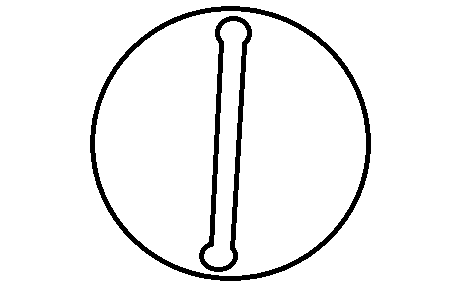
\includegraphics{sphereNotSimple}\\
Вырежем из северного и южного полюсов сферы кружочки, а затем разрежем её от одного кружочка до другого. Этим действием мы немного изменили промежутки принимаемых углами $\varphi$ и $\theta$ значений в сферических координатах, к которым мы и перейдем. Таким образом, теперь промежутки допустимых значений:\\
$$\frac{1}{n} \leq \varphi \leq 2 \pi - \frac{1}{n}$$
$$\frac{1}{n} \leq \theta \leq \pi - \frac{1}{n}$$
И теперь новая поверхность является простой.\\
\uline{Конус}:\\
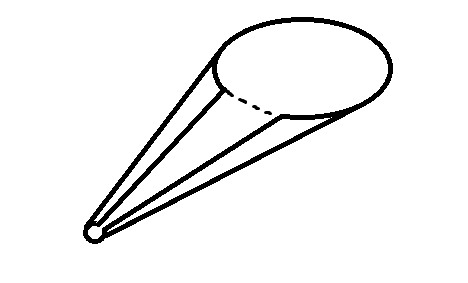
\includegraphics{coneNotSimple}\\
Вырежем вершину конуса и разрежем его по вертикали. Этим действием мы немного изменили промежутки допустимых значений для радиуса $r$ и угла $\varphi$ в цилиндрических координатах, к которым мы и перейдем. Таким образом, теперь промежутки допустимых значений:\\
$$\frac{1}{n} \leq r \leq n$$
$$\frac{1}{n} \leq \theta \leq 2 \pi - \frac{1}{n}$$
И теперь новая поверхность является простой.\\
\subsection{Функции, задающие одну и ту же поверхность}
Пусть даны $\Omega$ и $\Omega^{'}$, а так же соответствия $u=u(u^{'},v^{'}), v=v(u^{'},v^{'})$.\\
Кроме того, пусть якобиан $\begin{bmatrix} u_{u^{'}} & u_{v^{'}} \\ v_{u^{'}} & v_{v^{'}} \end{bmatrix}$ не равен 0 (то есть, существует обратная функция).\\
Это значит, что $\Omega$ отображается на $\Omega^{'}$ взаимно-однозначно.\\
В таком случае будем считать, что\\
$$\overrightarrow{r}(u,v) = \overrightarrow{r}(u(u^{'},v^{'}),v(u^{'},v^{'}))=\overrightarrow{\varrho}(u^{'},v^{'}) - \Sigma$$
(задают одну и ту же поверхность).\\
\subsection{Координатные кривые}
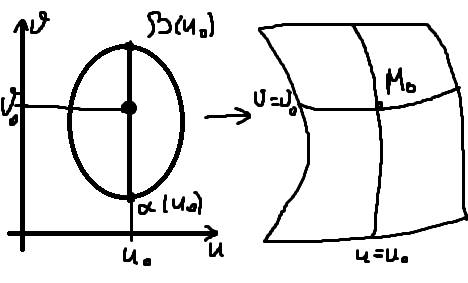
\includegraphics{coordCurves}\\
Зафиксируем одну из координат, например, $u=u_0$, и будем менять $v$ от $\alpha(u_0)$ до $\beta(u_0)$. Получим кривую $\overrightarrow{r}(u_0,v)$.\\
Аналогично, если зафиксировать $v=v_0$, то зададим кривую $\overrightarrow{r}(u,v_0)$.\\
Эти две кривые называются \textbf{координатными кривыми}.\\
\subsection{Нормаль}
Теперь рассмотрим $\overrightarrow{r}_u, \overrightarrow{r}_v$ - касательные к кривой.\\
Пусть $A = \begin{bmatrix}
   x_u & y_u & z_u \\
   x_v & y_v & z_v \\
\end{bmatrix}$, тогда если $rank A = 2$, то векторное произведение $\overrightarrow{r}_u \times \overrightarrow{r}_v \neq 0$.\\
Результат этого векторного произведения $\overrightarrow{r}_u \times \overrightarrow{r}_v = \overrightarrow{n}$ является вектором \textbf{нормали} к поверхности $\Sigma$.\\
Убедимся, что нормаль не зависит от параметризации кривой:\\
Дано взаимно-однозначное отображение $\Omega \iff \Omega^{'}$ и $\overrightarrow{r}(u,v) = \overrightarrow{\varrho}(u^{'},v^{'})$.\\
Посчитаем $\overrightarrow{\varrho}_{u^{'}} \times \overrightarrow{\varrho}_{v^{'}}$:\\
Вспомним, что $\overrightarrow{\varrho}(u^{'},v^{'}) = \overrightarrow{r}(u(u^{'},v^{'}),v(u^{'},v^{'}))$, это значит, что\\
$$\overrightarrow{\varrho}_{u^{'}} = \overrightarrow{r}_u \frac{\partial u}{\partial u^{'}} + \overrightarrow{r}_v \frac{\partial v}{\partial u^{'}},$$
$$\overrightarrow{\varrho}_{v^{'}} = \overrightarrow{r}_u \frac{\partial u}{\partial v^{'}} + \overrightarrow{r}_v \frac{\partial v}{\partial v^{'}}$$
Перемножим, учитывая, что векторное произведение коллинеарных векторов равно нулю:\\
$$\overrightarrow{\varrho}_{u^{'}} \times \overrightarrow{\varrho}_{v^{'}} = (\overrightarrow{r}_u \times \overrightarrow{r}_v) \frac{\partial u}{\partial u^{'}} \frac{\partial v}{\partial v^{'}} + (\overrightarrow{r}_v \times \overrightarrow{r}_u) \frac{\partial v}{\partial u^{'}} \frac{\partial u}{\partial v^{'}} = $$
$$ = (\overrightarrow{r}_u \times \overrightarrow{r}_v) (\frac{\partial u}{\partial u^{'}} \frac{\partial v}{\partial v^{'}}-\frac{\partial v}{\partial u^{'}} \frac{\partial u}{\partial v^{'}}) (\text{поменяли знак}) = (\overrightarrow{r}_u \times \overrightarrow{r}_v) \begin{bmatrix} u_{u^{'}} & u_{v^{'}} \\ v_{u^{'}} & v_{v^{'}} \end{bmatrix}$$
Но этот якобиан не равен нулю!\\
Это значит, что получили тот же вектор нормали, у которого могла измениться лишь длина или направление, что и требовалось доказать.\\
\subsection{Площадь поверхности}
Даны $\Omega, \overrightarrow{r}=\overrightarrow{r}(u,v)$.\\
Найдем дифференциал этого вектора:\\
$$d \overrightarrow{r} = \overrightarrow{r}_u du + \overrightarrow{r}_v dv$$
$$d \overrightarrow{r}^2 = |d \overrightarrow{r}|^2 = \overrightarrow{r}_u^2 du^2 + 2 \overrightarrow{r}_u \overrightarrow{r}_v dudv + \overrightarrow{r}_v^2 dv^2$$
Обозначим $E = \overrightarrow{r}_u^2, F = \overrightarrow{r}_u \overrightarrow{r}_v, G = \overrightarrow{r}_v^2$.\\
$d \overrightarrow{r}^2$ называется первой квадратичной формой поверхности и для неё справедливо свойство:\\
$d \overrightarrow{r}^2 > 0$ (положительно определена)ю\\
Для того, чтобы это выполнялось (для нашей формы $ax^2 + 2bxy + cy^2$), нужно:\\
$$\begin{cases} a > 0 \\ c > 0 \\ ac - b^2 > 0 \end{cases}$$
В нашем случае второго дифференциала вектора $\overrightarrow{r}$ это значит, что требуется выполнение следующих условий:\\
$$\begin{cases} E > 0 \\ G > 0 \\ EG - F^2 > 0 \end{cases}$$
Первые два условия очевидны, проверим третье:\\
$$| \overrightarrow{r}_u \times \overrightarrow{r}_v | = |\overrightarrow{r}_u| |\overrightarrow{r}_v| \sin \varphi \  (\varphi \neq 0)$$
$$\overrightarrow{r}_u \cdot \overrightarrow{r}_v = |\overrightarrow{r}_u| |\overrightarrow{r}_v| \cos \varphi$$
$$|\overrightarrow{r}_u \times \overrightarrow{r}_v|^2 + (\overrightarrow{r}_u \cdot \overrightarrow{r}_v)^2 = |\overrightarrow{r}_u|^2 |\overrightarrow{r}_v|^2$$
Заметим, что правая часть это $EG$, а второе слагаемое в левой части это $F^2$.\\
Тогда $|\overrightarrow{r}_u \times \overrightarrow{r}_v|^2 = EG-F^2 > 0$, так как $\overrightarrow{r}_u \times \overrightarrow{r}_v \neq 0$, что и требовалось доказать.\\
\uline{\textbf{Площадь поверхности}}\\\\
$S(\Sigma) = \iint_\Omega |\overrightarrow{r}_u \times \overrightarrow{r}_v| \ du dv$ - площадь поверхности.\\
Свойства площади:\\
1) Не зависит от параметризации.\\
Пусть дали две параметризации:\\
$$\overrightarrow{r}(u,v) = \overrightarrow{\varrho}(u^{'},v^{'})$$
$$S(\Sigma) = \iint_{\Omega^{'}} |\overrightarrow{\varrho}_{u^{'}} \times \overrightarrow{\varrho}_{v^{'}}| \ du^{'} dv^{'}$$
Вспомним, что $|\overrightarrow{\varrho}_{u^{'}} \times \overrightarrow{\varrho}_{v^{'}}| = |(\overrightarrow{r}_u \times \overrightarrow{r}_v)| \ |I(\frac{u,v}{u^{'},v^{'}})|$.\\
Подставим это в интеграл:\\
$$S(\Sigma) = \iint_{\Omega^{'}} |\overrightarrow{r}_u \times \overrightarrow{r}_v| \ |I| du^{'} dv^{'} = \iint_\Omega |\overrightarrow{r}_u \times \overrightarrow{r}_v| \ dudv$$
Получили то же самое.\\
2) Рассмотрим случай, когда сама поверхность - плоскость. Сможем ли по той же формуле посчитать площадь? Проверим это, площадь это $\iint_\Omega \ dudv$.\\
Теперь посчитаем $S(\Omega):$\\
$\Sigma$ задается при помощи $\overrightarrow{r} = (x,y,0)$.\\
Тогда $\overrightarrow{r}_x = (1,0,0)$\\
$\indent \overrightarrow{r}_y = (0,1,0)$.\\
А $\overrightarrow{r}_x \times \overrightarrow{r}_y = \begin{bmatrix} i & j & k \\ 1 & 0 & 0 \\ 0 & 1 & 0 \end{bmatrix} = \overrightarrow{k}, \Rightarrow |\overrightarrow{r}_x \times \overrightarrow{r}_y | = 1$.\\
Тогда $S(\Sigma) = \iint_\Omega |\overrightarrow{r}_x \times \overrightarrow{r}_y| \ du dv = \iint_\Omega du dv$, что и требовалось доказать.\\
3) Площадь аддитивна по отношению к поверхности. (Площадь поверхности, составленной из гладких кусков, равно сумме площадей).\\
4) $z = f(x,y)$.\\
$\overrightarrow{r} = (x,y,f(x,y))$.\\
$\overrightarrow{r}_x = (1,0,f_x)$.\\
$\overrightarrow{r}_y = (0,1,f_y)$.\\
$\overrightarrow{r}_x \times \overrightarrow{r}_y = \begin{bmatrix} i & j & k \\ 1 & 0 & f_x \\ 0 & 1 & f_y \end{bmatrix} = i (-f_x) - j f_y + \overrightarrow{k}$.\\
$$|\overrightarrow{r}_x \times \overrightarrow{r}_y| = \sqrt{EG - F} = \sqrt{f_x^2 + f_y^2 +1}$$
\uline{\textbf{ПРИМЕРЫ:}}\\
1) Посчитать площадь:\\
$$x^2 + y^2 + z^2 - R^2,$$
где $z \geq 0$.\\
Это половина сферы, которую вырезает цилиндр:\\
$$x^2 + y^2 = Rx, \Rightarrow x^2 - Rx + \frac{x^2}{4} + y^2 = (\frac{R}{2})^2, \Rightarrow (x-\frac{R}{2})^2 + y^2 = (\frac{R}{2})^2$$
Это выглядит так:\\
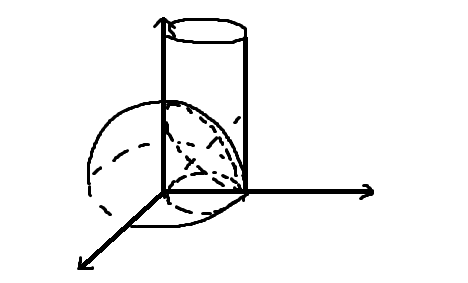
\includegraphics{halfSphereAndCylindr1}\\
Перейдем в сферические координаты:\\
$\begin{cases} x = R\cos\varphi \sin\theta \\ y = R \sin \varphi \sin \theta \\ z = R \cos \theta \end{cases}$.\\
Зададим поверхность:\\
$$\overrightarrow{r} = (R\cos\varphi \sin\theta, R\sin\varphi \sin\theta, R\cos\theta)$$
Посчитаем частные производные по $\varphi$ и $\theta$:\\
$\overrightarrow{r}_\varphi = (-R \sin \varphi \sin \theta, R\cos\varphi \sin \theta, 0)$\\
$\overrightarrow{r}_\theta = (R\cos\varphi \cos\theta, R\sin\varphi \cos\theta, -R\sin\theta)$\\
Теперь посчитаем $E, F, G$:\\
$E = \overrightarrow{r}_\varphi^2 = R^2 \sin^2 \varphi \sin^2 \theta + R^2 \cos^2 \varphi \sin^2 \theta = R^2 \sin^2 \theta$.\\
$F = \overrightarrow{r}_\theta^2 = R^2 \cos^2 \varphi \cos^2 \theta + R^2 \sin^2 \varphi \cos^2 \theta + R^2 \sin^2 \theta = R^2$.\\
$F = 0$ (если раскрыть скобки, то и правда получится 0).\\
$\sqrt{EG-F^2} = R^2 \sin\theta$.\\
Тогда $S(\Sigma) = \iint_\Omega R^2 \sin\theta \ d\varphi d\theta = 2 R^2 \int_0^{\frac{\pi}{2}} d\varphi \int_0^? \sin\theta \ d\theta$.\\
Осталось вычислить верхний предел интегрирования для $\theta$, для этого нужно подставить сферические координаты в уравнение цилиндра:\\
$R^2 \cos^2 \varphi \sin^2 \theta + R^2 \sin^2 \varphi \sin^2\theta = R^2 \cos\varphi \sin\theta$.\\
Отсюда либо $\sin\theta = 0$, либо $\sin\theta = \cos\varphi$.\\
Первое нас не интересует, а вот второе можно решить и получить ответ:\\
$\theta = \frac{\pi}{2} - \varphi$.\\
Тогда $S(\Sigma) = \iint_\Omega R^2 \sin\theta \ d\varphi d\theta = 2 R^2 \int_0^{\frac{\pi}{2}} d\varphi \int_0^{\frac{\pi}{2} - \varphi} \sin\theta \ d\theta = R^2(\pi - 2)$.\\
2) Посчитать площадь поверхности:\\
$z = x^2 + y^2$. Этот параболоид бесконечен, поэтому чтобы было, что считать, вырежем из него кусок $x^2 + y^2 = R^2$ и найдем площадь.\\
Вот как это выглядит:\\
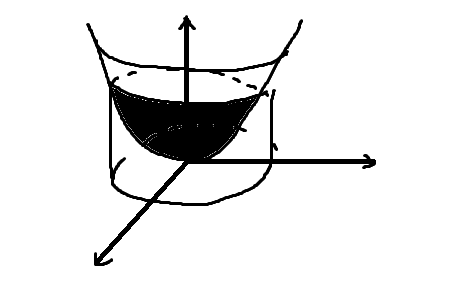
\includegraphics{paraboloidAndCylindr1}\\
Для этого перейдем к цилиндрическим координатам:\\
$\begin{cases} x=\varrho \cos \varphi \\ y = \varrho \sin \varphi \\ z = \varrho^2 \end{cases}$.\\
Зададим поверхность:\\
$\overrightarrow{r} = (\varrho\cos\varphi, \varrho\sin\varphi, \varrho^2)$.\\
Посчитаем частные производные по $\varrho$ и $\varphi$.\\
$\overrightarrow{r}_\varrho = (\cos\varphi, \sin\varphi, 2\varrho)$.\\
$\overrightarrow{r}_\varphi = (-\varrho\sin\varphi, \varrho\cos\varphi, 0)$.\\
Теперь посчитаем $E, F, G$:\\
$E = \overrightarrow{r}_\varrho^2 = 1 + 4 \varrho^2$.\\\\
$F = \overrightarrow{r}_\varphi^2 = \varrho^2$.\\
$F = 0$ (если раскрыть скобки, то и правда получится 0).\\
$\sqrt{EG-F^2} = \varrho\sqrt{1+4\varrho^2}$.\\
$$S(\Sigma)=\iint_\Omega \varrho\sqrt{1+4\varrho^2} \ d\varrho d\varphi = \int_0^{2\pi} d\varphi \int_0^R \varrho\sqrt{1+4\varrho^2} \ d\varrho$$
\uline{Важная информация про почти простые поверхности:}\\
Если $\Sigma$ - почти простая, а $\Omega_n$ - искомая исчерпывающая последовательность, то:\\
$$S(\Sigma) = \iint_\Omega |\overrightarrow{r}_u \times \overrightarrow{r}_v| \ dudv = \lim_{n\to\infty} \iint_{\Omega_n} |\overrightarrow{r}_u \times \overrightarrow{r}_v| \ dudv$$
\section{Поверхностные интегралы}
\subsection{Поверхностный интеграл первого рода}
Пусть $\Sigma$ - простая и гладкая поверхность. Дана $F(x,y,z)$ - непрерывная функция, определенная на $\Sigma$.\\
Поверхностным интегралом $\Romannum{1}$ рода от функции $F$ по поверхности $\Sigma$ называется:\\
$$\iint_\Omega F(x(u,v),y(u,v),z(u,v)) | \overrightarrow{r}_u \times \overrightarrow{r}_v| \ dudv = \iint_\Sigma F(x,y,z) ds (d\sigma)$$
\uline{Свойства поверхностного интеграла $\Romannum{1}$ рода:}\\
1) Не зависит от параметризации поверхности (доказывается так же, как независимость площади поверхности от параметризации).\\
2) Аддитивность и линейность.\\
3) Можно дать физическую интерпретацию:\\
Если $F(x,y,z) \geq 0$, и это плотность слоя, ''намазанного'' на поверхность, то $\iint F d\sigma$ - масса слоя.\\
\textbf{Вместо $d\sigma$ можно написать $\sqrt{EG-F^2} \ dudv$}.\\
\subsection{Поверхностный интеграл второго рода}
Пусть $\Sigma$ - двусторонняя (бывают односторонние поверхности, например, лист Мёбиуса и бутылка Клейна (Кляйна)). Выберем сторону (это означает, выберем, куда ''смотрит'' нормаль).\\
У нас есть поверхностный интеграл $\iint_\Sigma (\overrightarrow{F}, \overrightarrow{n}_0) \ d\sigma$, где $\overrightarrow{F} = (P(x,y,z),Q(x,y,z),R(x,y,z))$.\\
Если поменять сторону, то поменяется знак за счёт смены направления вектора нормали на противоположное.\\
Отсюда вытекает свойство:\\
$$\iint_\Sigma (\overrightarrow{F}, \overrightarrow{n}_0) \ d\sigma = -\iint_\Sigma (\overrightarrow{F}, \overrightarrow{n}_0^{-}) \ d\sigma$$
\subsection{Как считать поверхностный интеграл второго рода}
Рассмотрим $(\overrightarrow{F}, \overrightarrow{n}_0) = \overrightarrow{F} \frac{\overrightarrow{r}_u \times \overrightarrow{r}_v}{|\overrightarrow{r}_u \times \overrightarrow{r}_v|} \ |\overrightarrow{r}_u \times \overrightarrow{r}_v| \ dudv = (\overrightarrow{F} \cdot \overrightarrow{r}_u \cdot \overrightarrow{r}_v) \ dudv$ (смешанное произведение).\\
Посчитаем его:\\
$$\begin{bmatrix} R & Q & R \\ x_u & y_u & z_u \\ x_v & y_v & z_v \end{bmatrix} \ dudv = (P \frac{\partial (y,z)}{\partial(u,v)} + Q \frac{\partial (z,x)}{\partial(u,v)}\text{(поменяли знак)} + R\frac{\partial (x,y)}{\partial(u,v)}) \ dudv$$
Рассмотрим $PI (\frac{y,z}{u,v}) \ du dv$:\\
Если угол между вектором нормали и осью $x$ острый, то $I > 0$, иначе $I < 0$.\\
Тогда для острого угла $\iint PI \ du dv = \iint_{D_{yz}} P (x(y,z),y,z) \ dydz$.\\
А для тупого угла $\iint PI \ du dv = - \iint_{D_{yz}} P (x(y,z),y,z) \ dydz$.\\
Аналогично и другие слагаемые, тогда запишем сумму:\\
$P \frac{\partial (y,z)}{\partial(u,v)}\ dudv + Q \frac{\partial (z,x)}{\partial(u,v)}\ dudv + R\frac{\partial (x,y)}{\partial(u,v)} \ dudv = P\ dydz + Q\ dzdx + R \ dxdy$.\\
Тогда\\
$$\iint_\Sigma (\overrightarrow{F}, \overrightarrow{n}_0) \ d\sigma = \iint_\Sigma P \ dydz + Q \ dzdx + R \ dxdy$$
\uline{\textbf{ПРИМЕР:}}\\
Дан $\iint_\Sigma x \ dydz$, и вырезан прямоугольник $z + y - z = 1$, верхняя сторона.\\
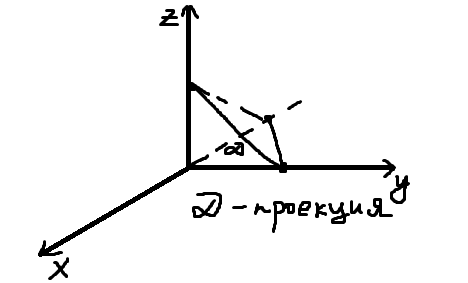
\includegraphics{triangleCut1}
Посчитаем:\\
$\iint_\Sigma x \ dydz = - \iint (z+y-1)\ dydz$ (так как угол между нормалью и отсутствующей осью (в данном случае ось $x$) тупой).\\
$$- \iint (z+y-1)\ dydz = - \int_0^1 dy \int_0^{1-y}(z+(y-1))\ dz = \frac{1}{6}$$
\section{Теория поля}
$\Omega \subset R^3$.\\
\Romannum{1}. Скалярное поле.\\
Если $\forall M \in \Omega \ \exists f(M)$ - число, тогда у нас на области $\Omega$ задано скалярное поле $f(M) = f(x,y,z)$.\\
\uline{Дифференцируемость.}\\
Будем называть $f(M)$ дифференцируемым в точке $M_0$, если существует такой вектор $\overrightarrow{c}$, что\\
$${\bigtriangleup f}(M_0) = {\bigtriangleup \overrightarrow{r}} \cdot \overrightarrow{c} + o(||\overrightarrow{MM_0}||)$$
$$\overrightarrow{c} = grad f(M_0) = (\frac{\partial f(M_0)}{\partial x}, \frac{\partial f(M_0)}{\partial y}, \frac{\partial f(M_0)}{\partial z})$$
Гуманитарии могут делать так:\\
$sinx + cosx = (sin+cos)x$.\\
Мы сделаем так для градиента, но осознанно и опираясь на законы:\\
$$(\frac{\partial f}{\partial x},\frac{\partial f}{\partial y}, \frac{\partial f}{\partial z}) = (\frac{\partial}{\partial x},\frac{\partial}{\partial y},\frac{\partial}{\partial z})f$$
Обозначим теперь $(\frac{\partial}{\partial x},\frac{\partial}{\partial y},\frac{\partial}{\partial z})$ за $\bigtriangledown$ (произносится ''набла'').\\
Это символический вектор, его координаты это вроде числа, но на самом деле, эта набла - целиком оператор и применяется к чему-то.\\
Тогда $(\frac{\partial f}{\partial x},\frac{\partial f}{\partial y}, \frac{\partial f}{\partial z}) = {\bigtriangledown f}$.\\
$\overrightarrow{c} = {\bigtriangledown f}$, тогда\\
$${\bigtriangleup f} = {\bigtriangleup \overrightarrow{r}} \cdot {\bigtriangledown f} = ({\bigtriangleup \overrightarrow{r}} \cdot {\bigtriangledown})f + o(||\overrightarrow{MM_0}||)$$
\uline{Производная по направлению.}\\
$$\frac{\partial f (M_0)}{\partial l} = \lim{t\to 0} \frac{f(M_0+t\overrightarrow{l_0})-f(M_0)}{\partial t}$$
Здесь $t > 0$, а $\overrightarrow{l_0}$ - орт направления.\\
Заметим, что числитель - приращение, так что можно переписать в виде:\\
$$\frac{\partial f (M_0)}{\partial l} = \lim{t\to 0} \frac{(t \overrightarrow{l_0} \cdot \bigtriangledown + o(t)}{\partial t} = (\overrightarrow{l_0} \cdot \bigtriangledown)f$$
\Romannum{2}. Векторное поле.\\
Если $\forall M \in \Omega \ \exists \overrightarrow{a}(M) = (P(x,y,z),Q(x,y,z),R(x,y,z))$, тогда на области $\Omega$ задано векторное поле $\overrightarrow{a}(M) = (P(x,y,z),Q(x,y,z),R(x,y,z))$.\\
\uline{Дифференцируемость.}\\
Будем называть $\overrightarrow{a}(M)$ дифференцируемым в точке $M_0$, если его приращение можно представить в виде:\\
$${\bigtriangleup \overrightarrow{a}(M)} = \overrightarrow{a}(M) - \overrightarrow{a}(M_0) = L(\overrightarrow{r})+o(||\overrightarrow{r}||)$$
Тогда\\
$${\bigtriangleup \overrightarrow{a}(M)} = ({\bigtriangleup \overrightarrow{r}} \cdot \bigtriangledown)\overrightarrow{a} + o(||\overrightarrow{r}||)$$
\uline{Производная по направлению.}\\
$\frac{\partial f}{\partial l} = (\overrightarrow{l_0} \cdot \bigtriangledown)f$ - для скалярного поля. В случае векторного поля:\\
$$\frac{\partial \overrightarrow{a}}{\partial l} = (\overrightarrow{l_0} \cdot \bigtriangledown)\overrightarrow{a}$$
\uline{\textbf{ПРИМЕР:}}\\
$\overrightarrow{a} = y \overrightarrow{i} + (xy + yz)\overrightarrow{j} + xyz \overrightarrow{k}$\\
$\overrightarrow{l} = (1,1,1), \overrightarrow{l_0} = (\frac{1}{\sqrt{3}},\frac{1}{\sqrt{3}},\frac{1}{\sqrt{3}})$\\
$\frac{\partial \overrightarrow{a}}{\partial l} = (\overrightarrow{l_0} \cdot \bigtriangledown)\overrightarrow{a}$\\
1) $(\overrightarrow{l_0} \cdot \bigtriangledown)\overrightarrow{a} = \frac{1}{\sqrt{3}} \frac{\partial}{\partial x} + \frac{1}{\sqrt{3}} \frac{\partial}{\partial y} + \frac{1}{\sqrt{3}} \frac{\partial}{\partial z}$, и все это нужно применить к вектору $\overrightarrow{a}$.\\
2) $(\overrightarrow{l_0} \cdot \bigtriangledown)\overrightarrow{a}$ - рассмотрим результат покоординатно:\\
$(\overrightarrow{l_0} \cdot \bigtriangledown)a_x = (\frac{1}{\sqrt{3}} \frac{\partial}{\partial x},\frac{1}{\sqrt{3}} \frac{\partial}{\partial y},\frac{1}{\sqrt{3}} \frac{\partial}{\partial z})y = \frac{1}{\sqrt{3}}$\\
$(\overrightarrow{l_0} \cdot \bigtriangledown)a_y = (\frac{1}{\sqrt{3}} \frac{\partial}{\partial x},\frac{1}{\sqrt{3}} \frac{\partial}{\partial y},\frac{1}{\sqrt{3}} \frac{\partial}{\partial z})(xy+yz) = \frac{2y+x+z}{\sqrt{3}}$\\
$(\overrightarrow{l_0} \cdot \bigtriangledown)a_z = (\frac{1}{\sqrt{3}} \frac{\partial}{\partial x},\frac{1}{\sqrt{3}} \frac{\partial}{\partial y},\frac{1}{\sqrt{3}} \frac{\partial}{\partial z})(xy) = \frac{yz+xz+xy}{\sqrt{3}}$\\
Тогда\\
$(\overrightarrow{l_0} \cdot \bigtriangledown)\overrightarrow{a} = \frac{1}{\sqrt{3}}\overrightarrow{i} + \frac{2y+x+z}{\sqrt{3}}\overrightarrow{j} + \frac{yz+xz+xy}{\sqrt{3}}\overrightarrow{k}$.\\
\uline{Введем понятия:}\\
Пусть дано поле $\overrightarrow{a} = \overrightarrow{a}(M) = (P,Q,R)$.\\
Тогда \textbf{дивергенция} поля:\\
$$div\overrightarrow{a} = \frac{\partial P}{\partial x} + \frac{\partial Q}{\partial y} + \frac{\partial R}{\partial z}$$
\textbf{Ротор} векторного поля:\\
$$rot\overrightarrow{a} = det \begin{bmatrix} i & j & k \\ \frac{\partial}{\partial x} & \frac{\partial}{\partial y} & \frac{\partial}{\partial z} \\ P & Q & R \end{bmatrix} = \overrightarrow{i} (\frac{\partial R}{\partial y} - \frac{\partial Q}{\partial z}) + \overrightarrow{j}(\frac{\partial P}{\partial z} - \frac{\partial R}{\partial x}) + \overrightarrow{k}(\frac{\partial Q}{\partial x} - \frac{\partial P}{\partial y})$$
Упростим формулы для $div$ и $rot$:\\
$div \overrightarrow{a} = (\bigtriangledown \cdot \overrightarrow{a})$ (скалярное произведение).\\
$rot \overrightarrow{a} = (\bigtriangledown \times \overrightarrow{a})$ (векторное произведение).\\
\uline{\textbf{Действия с $\bigtriangledown$}}:\\
1) $$\bigtriangledown(c_1 f_1 + c_2 f_2) = c_1 {\bigtriangledown f_1} + c_2 {\bigtriangledown f_2}$$
2) Посчитаем $\bigtriangledown(f_1 f_2)$:\\
$$\frac{\partial}{\partial x}(f_1 f_2) = \frac{\partial f_1}{\partial x} f_2 + \frac{\partial f_2}{\partial x} f_1$$
$$\frac{\partial}{\partial y}(f_1 f_2) = \frac{\partial f_1}{\partial y} f_2 + \frac{\partial f_2}{\partial y} f_1$$
$$\frac{\partial}{\partial z}(f_1 f_2) = \frac{\partial f_1}{\partial z} f_2 + \frac{\partial f_2}{\partial z} f_1$$
Будем иметь ввиду, что $\bigtriangledown$ действует на поле, когда пишем следующим образом:\\
$$\bigtriangledown(\overset{\downarrow}{f_1} f_2)$$
Здесь $\bigtriangledown$ действует на поле $f_1$.\\
Тогда $\bigtriangledown(f_1 f_2) = \bigtriangledown(\overset{\downarrow}{f_1} f_2) + \bigtriangledown(f_1 \overset{\downarrow}{f_2}) = f_1 {\bigtriangledown f_2} + f_2 {\bigtriangledown f_1}$.\\
3) Посчитаем $\bigtriangledown(\overrightarrow{a_1} \times \overrightarrow{a_2})$:\\
Формально это смешанное произведение, тогда\\
$$\bigtriangledown(\overrightarrow{a_1} \times \overrightarrow{a_2}) = \bigtriangledown(\overset{\downarrow}{\overrightarrow{a_1}} \times \overrightarrow{a_2}) + \bigtriangledown(\overrightarrow{a_1} \times \overset{\downarrow}{\overrightarrow{a_2}}) = \overrightarrow{a_2}(\bigtriangledown \times \overrightarrow{a_1})-\overrightarrow{a_1}(\bigtriangledown \times \overrightarrow{a_2})$$
4) $grad \ f = {\bigtriangledown f}$\\
5) $grad \ (f_1 f_2) = f_1 grad \ f_2 + f_2 grad \ f_1$\\
6) $div \overrightarrow{a} = \bigtriangledown \cdot \overrightarrow{a}$\\
7) $rot \overrightarrow{a} = \bigtriangledown \times \overrightarrow{a}$\\
8) $div (f \cdot \overrightarrow{a}) = \bigtriangledown(f \cdot \overrightarrow{a}) = \bigtriangledown(\overset{\downarrow}{f} \cdot \overrightarrow{a}) + \bigtriangledown(f \cdot \overset{\downarrow}{\overrightarrow{a}}) =\overrightarrow{a} \bigtriangledown f + f \bigtriangledown \overrightarrow{a} = \overrightarrow{a} grad \ f + f div \overrightarrow{a}$\\
9) $div (\overrightarrow{a_1} \times \overrightarrow{a_2}) = \bigtriangledown(\overrightarrow{a_1} \times \overrightarrow{a_2}) = \bigtriangledown(\overset{\downarrow}{\overrightarrow{a_1}} \times \overrightarrow{a_2}) + \bigtriangledown(\overrightarrow{a_1} \times \overset{\downarrow}{\overrightarrow{a_2}}) = \overrightarrow{a_2}(\bigtriangledown \times \overrightarrow{a_1}) - \overrightarrow{a_1} (\bigtriangledown \times \overrightarrow{a_2}) = \overrightarrow{a_2} rot \overrightarrow{a_1} - \overrightarrow{a_1} rot \overrightarrow{a_2}$\\
10) $rot(f\overrightarrow{a}) = \bigtriangledown \times (f\overrightarrow{a}) = \bigtriangledown \times (\overset{\downarrow}{f}\overrightarrow{a}) + \bigtriangledown \times (f\overset{\downarrow}{\overrightarrow{a}}) = ({\bigtriangledown f}) \times \overrightarrow{a} + f(\bigtriangledown \times \overrightarrow{a})  = grad \ f \times \overrightarrow{a} + f \ rot \overrightarrow{a}$\\
11) $rot(\overrightarrow{a_1} \times \overrightarrow{a_2}) = \bigtriangledown (\overrightarrow{a_1} \times \overrightarrow{a_2}) = \bigtriangledown \overset{\downarrow}{\overrightarrow{a_1}} \times \overrightarrow{a_2} + \bigtriangledown \overrightarrow{a_1} \times \overset{\downarrow}{\overrightarrow{a_2}} = (\overrightarrow{a_2} \bigtriangledown)\overrightarrow{a_1} - \overrightarrow{a_2}(\bigtriangledown \overrightarrow{a_1}) + \overrightarrow{a_1}(\bigtriangledown  \overrightarrow{a_2}) - (\overrightarrow{a_1} \bigtriangledown)\overrightarrow{a_2} = (\overrightarrow{a_2} \bigtriangledown)\overrightarrow{a_1} - \overrightarrow{a_2} div \overrightarrow{a_1} + \overrightarrow{a_1} div \overrightarrow{a_2} - (\overrightarrow{a_1} \bigtriangledown)\overrightarrow{a_2}$\\
12) $div (grad \ f) = \bigtriangledown \cdot ({\bigtriangledown f}) = \frac{\partial^2 f}{\partial x^2} + \frac{\partial^2 f}{\partial y^2} + \frac{\partial^2 f}{\partial z^2} = (\frac{\partial}{\partial x^2} + \frac{\partial}{\partial y^2} + \frac{\partial}{\partial z^2})f =\\= \bigtriangledown^2 f = \bigtriangleup f$.\\
$\bigtriangleup$ - оператор Лапласа, $\bigtriangleup = \bigtriangledown^2$.\\
13) $div (rot \overrightarrow{a}) = \bigtriangledown \cdot (\bigtriangledown \times \overrightarrow{a}) = 0$.\\
14) $rot (grad \ f) = \bigtriangledown \times (\bigtriangledown \cdot f) = 0$.\\
\textbf{\uline{Экскурс в физику - физический смысл ротора}}\\
Пусть дали твердое тело, оно вращается вокруг какой то оси, пусть по часовой стрелке:\\
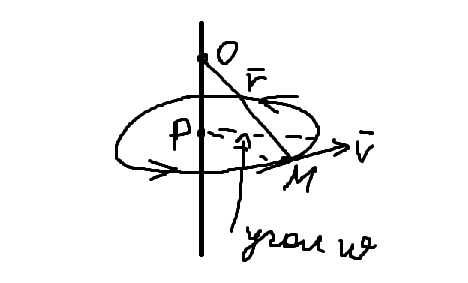
\includegraphics{rotorPhysicDefinition}\\
$|\overrightarrow{v}| = PM$(радиус)$\cdot \omega$.\\
Вектор $\overrightarrow{\omega} \times \overrightarrow{r}$ параллелен $\overrightarrow{v}$ (1)\\
$|\overrightarrow{v}| = \omega \cdot |\overrightarrow{r}| \sin \varphi = |\overrightarrow{\omega}| \ |\overrightarrow{r}| \sin (\pi - \varphi)$ (2)\\
Из (1) и (2) следует, что $\overrightarrow{v} = \overrightarrow{\omega} \times \overrightarrow{r}$.\\
Посчитаем $rot (\overrightarrow{v})$:\\
$rot(\overrightarrow{v})=rot(\overrightarrow{\omega} \times \overrightarrow{r}) = \overrightarrow{\omega} div \overrightarrow{r} - \overrightarrow{r} div \overrightarrow{\omega} + (\overrightarrow{r} \bigtriangledown) \overrightarrow{\omega} - (\overrightarrow{\omega} \bigtriangledown) \overrightarrow{r}$.\\
$\overrightarrow{\omega}$ зависит только от времени, следовательно, везде, где дифференцируем $\overrightarrow{\omega}$, будут нули:\\
$div \overrightarrow{\omega} = 0, (\overrightarrow{r} \bigtriangledown) \overrightarrow{\omega} = 0$.\\
Тогда $rot \overrightarrow{v} = \overrightarrow{\omega} div \overrightarrow{r} - (\overrightarrow{\omega} \bigtriangledown)\overrightarrow{r} = 3\overrightarrow{\omega} - \overrightarrow{\omega} = 2\overrightarrow{\omega}$.\\
Таким образом, физический смысл ротора: удвоенная мгновенная угловая скорость, отсюда и его названия (ротор, вихрь).\\
\section{Интегральные характеристики векторного поля}
Дано векторное поле $\overrightarrow{a} = \overrightarrow{a}(M)$ в $\Omega$, а так же $l$ - простой кусочно-гладкий замкнутый контур из $\Omega$.\\
\subsection{Циркуляция}
\textbf{Циркуляцией} векторного поля по замкнутому контуру $l$ называется следующий интеграл второго рода:\\
$$\text{Ц} = \int_l \overrightarrow{a} d\overrightarrow{r} = \int_l Pdx + Qdy + Rdz$$
\subsection{Поток}
Дана поверхность $\Sigma$.\\
\textbf{Потоком} векторного поля по поверхности $\Sigma$ называется следующий интеграл второго рода:\\
$$\prod = \iint_{\Sigma} \overrightarrow{a} \overrightarrow{n_0} ds$$
Приведем к привычному виду:\\
$$\prod = \iint_{\Sigma} \overrightarrow{a} \overrightarrow{n_0} ds = \iint_{\Sigma} Pdydz + Qdzdx + Rdxdy$$
\textbf{Физический смысл потока}\\
Пусть есть $\overrightarrow{a} = \overrightarrow{v}$ - поле скоростей. Жидкость движется по какому-то пути, а затем мы ставим на этом пути решетку:\\
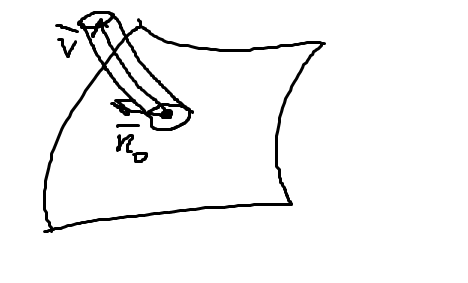
\includegraphics{currentPhysicDefinition}\\
И сколько жидкости проходит через решетку за единицу времени?\\
Возьмем в нашей решетке маленький кусок, из-за пренебрежимо малой величины можем считать его плоским. Тогда за единицу времени жидкость займет объем цилиндра с площадью основания, равной площади куска, и высотой, равной проекции $\overrightarrow{v}$ на ось вращения.\\
Посчитаем этот объем:\\
$$V_{\text{Ц}} = S \cdot |\overrightarrow{v}_{\text{пр.} \overrightarrow{n_0}}| = ds \overrightarrow{a} \overrightarrow{n_0} = d\prod$$
И поток будет равен приближенной сумме объемов по всем кусочкам, то есть интегралу.\\
\section{Теорема Гаусса-Остроградского (Остроградского-Гаусса)}
Пусть есть ограниченная область $\Omega \subset R^3$\\
Граница этой области - $\partial \Omega$ - кусочно-гладкая.\\
$\overrightarrow{n}$ - внешняя нормаль.\\
$\overrightarrow{a} = \overrightarrow{a} (M), M \in \overrightarrow{\Omega}, \overrightarrow{a}$ непрерывно дифференцируемо в каждой точке.\\
Тогда выполняется равенство:\\
$$\iint_{\partial\Omega} \overrightarrow{a} \overrightarrow{n_0} ds = \iiint_{\Omega} div \overrightarrow{a} dxdydz$$
Доказательство:\\
Предположим, что $\Omega$ односвязна и элементарна по всем координатам.\\
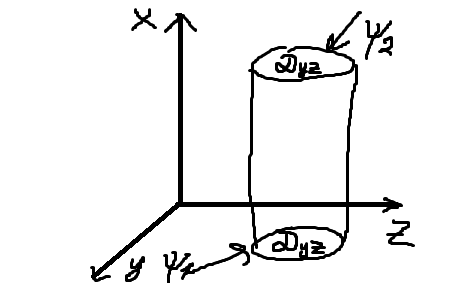
\includegraphics{ostrogradGaussProof}\\
Посчитаем одно из слагаемых, например, интеграл по $\frac{\partial P}{\partial x}$:\\
$\iiint_\Omega \frac{\partial P}{\partial x} dxdydz = \iint_{D_{yz}} dydz \int_{\psi_1(y,z)}^{\psi_2(y,z)} \frac{\partial P}{\partial x} =\\= \iint_{D_{yz}} P(\psi_2(y,z),y,z)dydz-\iint_{D_{yz}} P(\psi_1(y,z),y,z)dydz =\\= \iint_{\Sigma_1} P(x,y,z) dydz + \iint_{\Sigma_2} P(x,y,z) dydz + 0$ (интеграл по боковой поверхности равен нулю).\\
Здесь $\Sigma_1$ образована функцией $x = \psi_1(y,z)$, $\Sigma_2$ образована функцией $x = \psi_2(y,z)$.\\
Тогда эта сумма - интеграл по всей границе (три слагаемых это интеграл по верхней части, нижней части и боковой поверхности), а значит, она равна\\
$$\iint_{\partial \Omega} P(x,y,z) dydz$$
Аналогично доказывается для $Q$ и для $R$.\\
\end{document}